\chapter[Introduction]{Introduction}
\label{chap:chap1}
\section{Proposition}
\label{sec:chap1-motivation}
Purple phototrophic bacteria (PPB) have recently been proposed as an effective biotechnology for engineered applications including the treatment of domestic \cite{hulsen2016} and industrial wastewaters \cite{hulsen2018}. Phototrophic bacteria, have also shown promise in a range of highly valued end products such as animal feeds \cite{sun2016}, biofuels \cite{adessi2014}, and even cosmetic and pharmaceutical products\cite{liu2013, Wang2018}. Despite the increasing interest in these applications, they have not achieved widespread implementation largely due to the gaps in collective knowledge at the process level. In particular, the description and quantification of the interactions between biochemical behaviour, irradiation, and fluid hydrodynamics have proven to be significant design bottlenecks when scaling up photobioreactors. 
\skippingparagraph
Compared with iterative physical prototyping, semi-mechanistic modelling approaches can allow us to better understand these interactions. Using a modelling approach, exploring how performance and behaviour changes in response to different designs and operating conditions can aid in decision making as technologies increase in scale. As such, this thesis aims to explore the current state of process modelling, computational fluid dynamics, and radiative transfer modelling and combine these concepts into a unified distributed parameter modelling framework for phototrophic systems and photobioreactors.


%------------------------------------------------------------------------------%
%------------------------------------------------------------------------------%
%------------------------------------------------------------------------------%



%------------------------------------------------------------------------------%
%------------------------------------------------------------------------------%
\newpage
\section{Background}
\label{sec:chap1-background}
\subsection{Model types}
\label{ssec:chap1-wwtmod}
Models use mathematical expressions to explain the underlying processes or inputs of outputs of a system \cite{hangos2001}. They can be classed according to the method of their development. When developing process models, a number of decisions can be made depending on the nature of the model and the information required for understanding.
\begin{itemize}
    \item Mechanistic or empirical models
    \item Continuous or discrete models
    \item Lumped parameter (well-mixed) or distributed parameter models
    \item Stochastic or deterministic models
\end{itemize}

Mechanistic models are those which are based on known physical relationships. They differ from empirical models in that they are transparent; mechanisms are well known and well explained within the model. Empirical models are based on experimental results, and the mechanisms of the physical phenomena are not well captured by the model, and may not be reproducible under different environmental conditions. An example of a mechanistic and empirical model are Michaelis-Menten and Monod kinetics respectively. The former is based on the relationship between enzymatic processes and environmental substrate concentration, and the latter relate specific growth rate to environmental substrate concentration and the values can change based on surrounding conditions \cite{tchobanoglous1991}. Continuous models treat state variables as a lumped quantity such as concentration. If a state variable is non-denumerable, then it is continuous. On the other hand, discrete models consider denumerable quantities such as number of particles in a system, or a model of the number of exceedances of a certain pollutant emanating from a wastewater treatment plant \cite{hangos2001}. Lumped parameter models are those where the variations in space are assumed to be null, \ie the system is well-mixed such as a continuously stirred tank reactor. Solving a dynamic lumped system means that only a set of ordinary differential equations in time are required. Distributed parameter systems are therefore described by a set of partial differential equations \cite{hangos2001}. Stochastic models are those which incorporate randomness within the system whereas deterministic systems can be completely reproduced from the set of parameters, initial and boundary conditions. Stochastic models with identical initial and boundary conditions will lead to a multitude of different results often constrained by probability distributions \cite{voskoglou2007}. Most models are developed using a combination of these different categories, depending on the target use of the model.

\subsection{Modelling in wastewater}

Most of the available literature for wastewater treatment models is concerned with semi-mechanistic, continuous, lumped parameter and deterministic approaches to modelling. The major generic models in the domain of wastewater treatment, from which this thesis branches, are the International Water Association (IWA) family of models. These include the activated sludge model family, and the anaerobic digestion model (ADM) \cite{batstone2006} family. These have been combined together with appropriate unit process models such as clarifier models \cite{takacs1991} into standardised plant-wide models such as the benchmark simulation models (BSM1 and BSM2) \cite{jeppsson2007, beraud2007}. Modelling of wastewater treatment processes can lead to a greater understanding of the underlying physics and biochemistry \cite{szilvester2010}. All IWA models are semi-mechanistic, which means that the model equations are based on known mechanistic phenomena, such as the presence of known biological clades, but the kinetic relationships are generally empirical.
\skippingparagraph
The overarching goal of wastewater treatment is to protect public and environmental health. Regulators are placing increasing restrictions on wastewater effluent quality while influent characteristics are dynamic due to seasonality, weather, and other perturbations. Handling this uncertainty in input while achieving a reproducible effluent quality which meets licensing restrictions means that a deeper understanding of process mechanisms and uncertainty is required \cite{solon2019}.
Process models for wastewater treatment are good tools to address these restrictions and obligations. The benefits of these models are that they are readily extensible, and allow themselves to be used in distributed parameter models \cite{batstone2006a}. This also means that the IWA models can be applied for PPB time-series and distributed parameter models in contexts broader than just wastewater treatment. 



\subsubsection{Convergence of wastewater modelling standards}
\textbf{How did the models end up as grey box for biochemistry, and mechanistic for almost everything else. The work done by the IWA modelling task forces would go a long way to explaining this. }

\subsubsection{Purple phototrophic bacteria for wastewater treatment}
Purple phototrophic bacteria are some of the most metabolically versatile organisms on earth \cite{hunter2008}. They have been shown to grow well as photoheterotrophs under anaerobic conditions \cite{hulsen2014}. They also grow chemoheterotrophically in the absence of irradiation, and they grow photoautotrophically using irradiance to drive $\mathrm{CO_2}$ fixation \cite{gordon2014}. With respect to the modelling of phototrophic bacteria, there currently exist no models in the context of wastewater treatment and industrial growth in mixed systems on nutrients and organics, however the suite of metabolic modelling of PPB is rich but not readily applicable for a process engineering perspective \cite{klamt2002}.
\skippingparagraph
Phototrophic microorganisms pose promising solutions to current important technological challenges: the management of wastes such as atmospheric pollutants and wastewater, production of high value products from waste streams, such as biofuels and bio-plastics \cite{hulsen2016}. They are resilient under favourable radiative conditions, quickly out-competing other non photosynthetic organisms \cite{posten2009}. Photosynthetic and phototrophic microorganisms can be used in photobioreactors (PBR), which can be categorised based on whether the reactor is situated indoors or outdoors, its geometry (tubular, flat plate, raceway), whether it is anaerobic or aerobic, and the method of mixing (sparged, paddle wheel). The technology for these various applications has however not been widely adopted, partly due to gaps in understanding of good PBR design, and partly due to energy and utilities markets not being favourable to large scale implementations. A method to address the former is to undertake virtual prototyping using computational fluid dynamics CFD \cite{bitog2011}. This allows rapid development and experimentation, without the traditional expenses incurred in the scale up process \cite{bridgeman2012}.


\subsubsection{Purple phototrophic bacteria and radiation modelling}
PPB have evolved to efficiently harvest available solar radiation in aquatic environments \cite{cogdell2006}. Due to oxygenic photosynthetic organisms filtering radiation in the visible band in the upper aerobic zones of these aquatic systems, PPB have adapted to make use of remaining solar energy, which include green and near infra-red (NIR) radiation \cite{cogdell2006}. The light harvesting apparatus in \textit{Rhodobacterales} consists of two light harvesting complexes (LH2 and LH1), and a reaction centre (RC) \cite{hellingwerf1994}. A useful abstraction of the light harvesting complex is two distinct zones (LH2 and an LH2-RC complex) with absorbance spectra at 800-850 \si{nm} and 880 \si{nm} respectively. Figure \textbf{cite: figure} demonstrates how these light harvesting centres are arranged and how they participate in providing energy to the electron transport chain to ultimately generate ATP for growth and other cell processes.
\skippingparagraph
In terms of modelling PPB and their interactions with photons for industrial applications, very little has been done. Most studies focusing on photobioreactor design have been for hydrogen production applications \cite{adessi2014, krujatz2015}. Further limitations to these works were that particular wavelengths were not selected, with most opting for direct sunlight or white tungsten or halogen lamps as light sources. These approaches are problematic for a wastewater treatment application, as the use of broad spectrum light will leads to competition by other heterotrophic bacteria, and other phototrophic and photosynthetic organisms found in domestic wastewater such as algae and cyanobacteria.
\skippingparagraph

Efforts were made to combine a mass balance approach to the photoheterotrophic efficiency of PPB \cite{minkevich2004}. In this work, theoretical and experimental yields of purple phototrophic bacteria were calculated based on different electron donors and light sources. The maximum theoretical yields based on acetate as an electron donor are summarised in Table~\ref{tab:theoreticalQuantum}, where $Y^m_{X/LE}$ is the maximum biomass growth per light energy dose;

\begin{table}[H]
  \begin{center}
    \caption{Maximum theoretical \textit{Rb. capsulatus} yield with
      acetate as electron donor for different wavelengths
      \cite{minkevich2004}}
    \label{tab:theoreticalQuantum}
    \begin{tabular}{ | l | l |}
      \hline
      Wavelength& $Y^m_{X/LE}$ ($gVSS\cdot kJ^{-1}$)\\ \hline \hline
      860 nm & 0.020 \\ \hline
      744 nm & 0.017  \\ \hline
      522 nm & 0.012  \\ \hline
    \end{tabular}
  \end{center}
\end{table}

The theoretical model was then compared to experimental data, with the
following values obtained through experiment. This information is
presented in Table~\ref{tab:expQuantum}.

\begin{table}[H]
  \begin{center}
    \caption{PPB experimental yield for different wavelengths and
      lactate and acetate as electron donors\cite{minkevich2004}}
    \label{tab:expQuantum}
    \begin{tabular}{ | l | l | l | l |}
      \hline
      \textbf{Species} & \textbf{Wavelength} & \textbf{Electron donor} & $Y_{X/LE}$ ($gVSS\cdot kJ^{-1}$)\\ \hline \hline
      \textit{Rb. capsulatus} & 860 nm & lactate & 0.018 - 0.031 \\ \hline
      \textit{Rb. sphaeroides} & White ($\bar{\lambda}$ = 744 nm) & acetate & 0.009 - 0.016 \\ \hline
      \textit{Rb. capsulatus} & 522 nm & lactate & 0.006 - 0.013 \\ \hline

    \end{tabular}
  \end{center}
\end{table}
	
The data of \cite{minkevich2004} serves as an effective basis for quantifying and understanding the interactions between biomass growth, maintenance and decay, and the irradiance required for optimal reactor performance.


\subsection{Computational fluid dynamics for wastewater treatment and photobioreactors}
Traditional design methods of wastewater treatment process units consist of load and mass based static analysis, and testing of dynamic behaviour based on key operating state variables \cite{gaden2013}. Computational fluid dynamics (CFD) is a cost-effective method for scaling up process units and testing variations in operating parameters. This allows the design of equipment without needing physical prototypes \cite{wood1995}. CFD involves the spatiotemporal numerical analysis of transport equations and chemical reactions \cite{versteeg2007}. There have been many applications for CFD, including aerodynamic studies of aircraft, turbine analysis in power plants, environmental modelling of pollutants, and biomedical analysis of blood flows \cite{versteeg1995}. The major CFD studies in water treatment modelling have been conducted in the fields of algae growth, the inactivation of pathogens by ultraviolet radiation, and geometry and flow optimisation of conventional treatment plant units such as clarifiers, ponds and digesters. These areas of application have been chosen as a basis for literature review, due to photobioreactors operating with similar physical phenomena such as radiation delivery, multiphase fluid flows, and biochemical reactions \cite{bitog2011}. 

\subsubsection{CFD modelling of gas and liquid systems}
There are numerous studies looking at modelling bubble columns in a spatio-temporal manner. One of the early works in this field identified a need to consider a modelling technique incorporating spatio-temporal variations in order to minimise capital and operating costs during scale-up of general bubble column reactors \cite{lapin1994}. In this study, the Navier-Stokes system of equations modelled the continuous fluid phase, and the dispersed gas bubbles were modelled as discrete tracked particles, with their position being solved over time. As this was a 1994 study, the computing power limited the model development to a two dimensional 60 x 200 grid of a $0.75 m^{2}$ reactor face. Numerical diffusion arose when both the liquid and gas were considered as continuous phases. With the improvement in desktop computing capacity, CFD has been used extensively for bubble column and airlift reactor validation using both approaches \cite{bitog2011}. Other studies have looked at describing bubble flow within different reactor geometries with Eulerian-Eulerian (both phases considered continuous) methods \cite{lehr2002, pfleger2001, buwa2002, pareek2003, ekambara2005, sokolichin1999}. Gas-liquid flow in bubble columns has also been investigated with Eulerian-Lagrangian (continuous liquid phase and discrete gas phase) models \cite{zhang2013a}. The major works in this field have looked at different geometry bubble columns with drag force, virtual mass force, lift force primarily with two dimensional geometries \cite{buwa2006, goz2004, luo2011, ekambara2005, mouza2004}. These studies looked at the sensitivity of the columns to such parameters and conditions as turbulence model, sparger location, superficial gas velocity, reactor aspect ratio and virtual mass.
\skippingparagraph

The main strength of these bubble column CFD models is that they are applied to general simple geometries, as the main focus was to isolate the bubble flows to explain the effects of the principal hydrodynamic operating conditions and parameters. These general approaches to CFD modelling of bubble columns present a strong platform from which to commence photobioreactor simulations, but they also lead to limitations in the context of purple phototrophic bacteria for wastewater treatment. Even if solids are present in the system being modelled, phases are modelled as liquid and gas. Modelling approaches for solid phases require refinement, in which the solids are modelled as discrete particles, and the liquid and gas phases are modelled as continuous phases. In addition, these cases used simple geometries, which will probably not be appropriate for photobioreactor modelling and design, as the irradiated surface to volume ratio plays an important role in reactor performance \cite{soman2015}. Another note is that the generality of these cases means that biochemical reactions and photon-biomass interactions were not included in the studies. 


\subsubsection{Modelling of dispersed biosolid phases}
\label{S:21}
In general, there are two methodologies, Eulerian and Lagrangian, that can be implemented to solve the transport of a dispersed solid phase within continuous fluid phase(s) in a CFD simulation. The Eulerian approach treats the solid phase as a continuum and computes the concentration distribution based on the solution of a PDE that generally includes convective and diffusive terms, and may include various source and sink terms as required.  The Lagrangian approach, on the other hand, involves the calculation of a large number of particle trajectories, based on Newton's second law, and models of all forces acting on the particles, such as drag, lift, and gravity. Each method has its own advantages and disadvantages, and, depending on the specific objectives of the study, one method may be more appropriate or efficient than the other.  After outlining the details of each, recommendations will be made regarding the suitability of each for modelling PBR systems.
\skippingparagraph
In the Eulerian modelling approach, the flow field and concentration distribution of the particulate phase are calculated in sequence.  The PDE governing the particle phase concentration is \cite{zhang2007} (add more references)

%%%%%%%%%%%%%%%%%%%%%%%%%%%%%%%%%%%%%%%%%%%%%%%%%%%%%%%%%%%%%%%%%%%%%%%%%%%%
%      INSERT THE EULERIAN PDE FOR PARTICLE PHASE CONCENTRATION 
%%%%%%%%%%%%%%%%%%%%%%%%%%%%%%%%%%%%%%%%%%%%%%%%%%%%%%%%%%%%%%%%%%%%%%%%%%%%
\begin{equation}
\frac{\partial C}{\partial t}
+ \nabla\cdot\left(\mathbf{u} C\right)
= \Gamma\nabla^2 C
+ S_c
\label{eq:eulerian_pde}
\end{equation}

The second term on the left side of Eq.\ \ref{eq:eulerian_pde} represents convection of the particles with the velocity of the fluid phase(s), coupling the flow and concentration fields.  This coupling is one-way since the solids concentration does not influence the flow field.  The first term on the right side of Eq.\ \ref{eq:eulerian_pde} represents diffusion, while the second term represents all sources and sinks.

%
\begin{equation}
	\frac{d\mathbf{u}_p}{dt}
    = F_D\left(\mathbf{u}-\mathbf{u}_P\right)
    + g\frac{\rho_p-\rho}{\rho_p}
    + \mathbf{F}_a
	\label{eq:lagrangian_ode}
\end{equation}

\subsubsection{Comparison of Eulerian and Lagrangian Methodologies}

The Eulerian and Lagrangian approaches have been compared previously for particle transport in enclosed air spaces \cite{zhang2007}. Here the comparison is considered specifically in the context of PBR systems.


\skippingparagraph
The use of CFD for PBR analysis has increased since the first few studies in the early 1980s \cite{patankar1980}. Wider access to commercial CFD software packages and suitable computational resources are likely factors in this uptake. Commercial packages allow the user to streamline the work flow from geometry design, to meshing, to case set up, to data analysis and visualisation. One must however be prudent when carrying out CFD studies of PBRs, because the automation and ease in setting up cases with commercial packages could lead to undesirable or even non-validated and inaccurate solutions. Such issues of good CFD modelling practice and uncertainty quantification have been well documented in industries with a longer history of CFD usage \cite{roache2002,oberkampf2002,celik2008,pelletier2010}.  More recently, efforts have been made to outline good CFD modelling practices in the context of wastewater treatment plants \cite{wicklein2016}.
\skippingparagraph

CFD modelling has aided in the understanding of hydrodynamic processes, and a comprehensive review was carried out in 2011 reflecting the status of CFD modelling of PBRs \cite{bitog2011}. Most papers reviewed focused on the implications of certain geometry designs on flow characteristics. The papers were sampled to find a consensus on the use of a turbulence model. It was found that all studies reported used Reynolds-average Navier-Stokes (RANS) models, with the most popular being the standard $k-\epsilon$ model. The popularity of RANS models is not surprising, owing to their efficiency compared to more complex turbulence models.  The ubiquitous use of the standard $k-\epsilon$ model is somewhat surprising, given the evidence which shows this model is quite poor in predicting separated flows \cite{menter2003}. Further, it is clear that improved $k-\epsilon$ models, such as the realisable $k-\epsilon$ model \cite{shih1995}, as well as other improved RANS models, such as the $k-\omega$  SST model \cite{menter1994,menter2003} have been developed to address such deficiencies.
\skippingparagraph

The goal of this review is to not only provide an update in the state of the art CFD modelling practices, but to focus on the coupling and interactions between pertinent physical phenomena in PBR systems. Categories have been organised based on these physical processes, including hydrodynamics, radiation, biokinetics, porous media modelling for membrane and biofilm systems, and attempts to couple these processes. In addition, attention must be paid to analytical approaches including discretisation error evaluation. Guidelines from the Journal of Fluids Engineering can be adapted to this review \cite{celik2008}.
\skippingparagraph

This work is based the recommendations presented by \cite{posten2009}, and will assess CFD for PBR based on the following performance indicators that were highlighted: mixing, ``light'' delivery, mass transfer (including $CO_2$ delivery and $O_2$ purging in the case of micro-algae), and total energy demand. The study also alluded to the necessity in understanding and using the interactions between mass and radiative transfer, physiology of the microorganism in question, and their radiation and substrate kinetics and dynamics. In addition to these components, we have also identified that biofilm formation is important, whether one wants to avoid it, or use it as a design feature \cite{castro2017}.

\begin{itemize}
\item hydrodynamics, including mixing and mass transfer
\item radiative transfer
\item phyisiology and biokinetics
\item biofilms
\item methods for coupling all physical phenomena
\item analysis of error and grid convergence
\end{itemize}

The solution for the flow of a fluid is obtained by numerical solution of the Navier-Stokes equations, along with addition models, as required, to account for multiple phases, turbulence, etc. Most often, the equations are discretised using a finite volume method (FVM), but can also be discretised using other methods such as the finite element, finite difference, or spectral methods.  The most common CFD packages for PBR studies are ANSYS Fluent and ANSYS CFX, both of which are based on FVM.  Although it has not been used extensively for CFD analysis of PBRs, OpenFOAM is another FVM-based CFD code which is open source.


%---------------------------------------------------------------------------------------------------
%%%%%%%%%% RADIATION MODELLING
%---------------------------------------------------------------------------------------------------
\subsection{Radiation Modelling}
\label{S:radiation}
There are many approaches to modelling the radiation within photobioreactors, each with different levels of complexity and effectiveness. The general form of the radiative transfer equation (RTE) for a participating medium, upon which the approximations are based, is as follows \cite{modest2003}:

\begin{align}
\frac{dI_\lambda (\mathbf{r}, \mathbf{s}) }{ds} &=  \kappa_{\lambda}I_{b\lambda} \, - \, (\kappa_\lambda + \sigma_{\lambda, s}) \ I_\lambda (\mathbf{r}, \mathbf{s}) \nonumber \\
&+ \frac{\sigma_{\lambda, s}}{4 \pi} \int_{4 \pi} I_\lambda (\mathbf{r}, \mathbf{s'}) \Phi_\lambda(\mathbf{s}, \mathbf{s'}) d\Omega'
\label{eq:RTE}
\end{align}


where;\\
$I_\lambda (\vec{r}, \vec{s})$ is the spectral intensity of a radiative ray [$W \cdot m^{-2}$]. \\
$\vec{r}$ is a position vector [$m$]. \\
$\vec{s} \, \vec{s'}$ are the radiation path direction and scattering direction respectively.\\
$\kappa_\lambda$ is the spectral absorption coefficient [$m^{-1}$]. \\
$\sigma_{\lambda, s}$ is the scattering coefficient [$m^{-1}$].  \\
$s$ is the path length [$m$]. \\
$\Phi_\lambda$ is the spectral scattering phase function. \\
$\Omega'$ is the solid angle. \\

The left hand side of the equation is the rate of change of intensity along a direction, the first term on the right hand side is extinction (absorption and scattering) of the radiative intensity ray, and the second term on the right hand side is the the gain due to in-scattering. Usually black body emission can be omitted from the RTE, as the phenomenon of interest is the growth of biomass aided by absorption of photons. Flow rates and any external heat sources usually allow us to neglect this term \cite{lee1994}.


%%%%%%%% Beer Lambert Law
\subsubsection{Beer-Lambert law}
\label{S:2.3.1}
Among the most simple of radiative field solution techniques is the Beer Lambert law, an explicit solution to spectral intensity through a first order approximation (equation \ref{eq:beerLambert}). 
\begin{equation}
\frac{I(x)}{I_0} =  exp(-\beta x)
\label{eq:beerLambert}
\end{equation}

where, $I(x)$ is the irradiance at point $x$, $I_0$ is the incident irradiance. This equation can be adapted to a spectral equation by noting the dependence of the extinction coefficient on the wavelength. It is then a matter of integrating these spectral incident intensities into a total incident irradiance (G) \cite{pottier2005}.
\skippingparagraph
This approach lumps the absorption ($\kappa_\lambda$) and out-scattering ($\sigma_\lambda$) coefficients into one extinction coefficient ($\beta_\lambda$). The attenuation of radiation is modelled as a function of path length, concentration of the participating medium, and the extinction coefficient. The major problem with the Beer-Lambert law is that it neglects the effects of in-scattering, which can potentially give discrepancies of 20\% in the final solution \cite{berberoglu2007,pottier2005,wang2014a}. This can be translated to an assumption of isotropic scattering. The optical thickness in photobioreactors is much greater than unity, meaning that the assumption of isotropic scattering does not hold \cite{modest2003}.
\skippingparagraph
The process for designing photobioreactors with CFD has been to solve the fluid fields and then overlay the Beer-Lambert field on the fluid solution to determine a photo history. One can then gain insight into the radiation history of phototrophic particles, an important design parameter. \cite{marshall2010} explored the effects of light attenuation and algal growth using a three dimensional Beer-Lambert law. The authors coupled the biomass growth to the radiation field as per the Eilers-Peeters model for photosynthetic biomass growth states as detailed in \cite{bechet2013}. Wavelengths corresponding to pigment absorption were not considered, but the terms in the Eilers-Peeters model are adaptable to particular phototrophic organisms, which could be understood as an implicit treatment of spectral radiation. A  also used simple Beer-Lambert law has also been used to solve the radiative field within a PBR \cite{nauha2013}, on the way to a more complex solution focusing on the interactions involved between fluid flow, radiation, and growth kinetics. Other studies involving coupling also involved a similar approach \cite{marshall2011}. 
\skippingparagraph
There are many examples of studies looking at the \textit{radiation history} of a phototrophic particle by solving the flow field and subsequently solving the radiative field. This approach works under the assumption that the hydrodynamic field is at steady state, and any fluctuations in flow do not lead to significant changes in biological growth. Particles are then introduced into the system, either as massless entrained particles, or as participating particles subjected to external forces \cite{zhang2013}. The movement of these particles into and out of light and dark regions of the reactor can be analysed for insight into the growth characteristics induced by PBR design and operating condition variations. Some studies looked at the attenuation of light by algae and $CO_2$ bubbles in a sparged bubble column PBR \cite{hochhalter2014}. Other formations include raceway ponds \cite{gharagozloo2014,Park2015}, and tubular photobioreactors with static mixers \cite{cheng2016}. CFD was used to determine the light field of a hydrogen producing photobioreactor with \textit{Rhodobacter sphaeroides} \cite{krujatz2015}. A cylindrical continuous stirred PBR was used as the test case. An empirical radiation expression was used in an attempt to better approximate the scattering processes within a reactor. The method was adapted from a previous study \cite{suh2003}. The following hyperbolic model with empirical attenuation parameters $K_l$, $K_c$ and $\epsilon_m$ relating to scattering due to the dry weight concentration of biomass ($c_{dw}$) and path length ($l$), and the extinction due to maximal absorption ($\epsilon_m$) is:


\begin{equation} 
\frac{I}{I_0} (c,l) = exp \left[\frac{\epsilon_m \, l \, }{(K_c + c_{dw})(K_l + l)}\right]
\end{equation}

This model holds under the assumption of monochromatic radiation. The purpose of this study was to carry out particle tracing simulations where the radiation history of the particle could be tracked over time with different impeller speeds. This allowed more control over interactions between photons and biomass, leading to a higher production of hydrogen with a lower impeller frequency. The simulations were not coupled to the biokinetics of the system. With the exception of \cite{gharagozloo2014,krujatz2015}, there were no clear efforts to separate the extinction coefficient into its absorption and scattering components. More accurate solutions which account for biological photon absorption, out-scattering, as well as in-scattering exist. These solutions are more general, leading to more adaptability when exploring different reactor configurations \cite{ho2009}.


\subsubsection{Radiative transfer equation discretisation approaches}
\label{S:2.3.2}
A potentially more accurate approach to determining the radiation field in a photobioreactor is to solve an approximation to the complete radiative transfer equation. Photons of particular frequency are absorbed by the pigments of phototrophic microorganisms \cite{mcdermott1995}. It is therefore important to consider the spectral nature of the radiation in order to develop a deeper understanding of how the incident radiation is attenuated by either biomass absorption, or scattered by other components in the participating medium. There are several methods used to discretise the RTE, including the P-1 approximation, the discrete ordinates method (DOM), the finite volume discrete ordinates method (FVDOM), the Monte Carlo (MC) method, and the flux approximation \cite{coelho2008}. Of this list of approaches, the DOM, FVDOM and MC methods allow for resolution of the total spectral radiative transfer equation on the existing mesh \cite{kong2014}. The best balance between computational effort and solution accuracy is the FVDOM \cite{modest2003,kong2014} . The FVDOM discretisation of the RTE shares a starting point with the DOM, with the angular discretisation being the point of difference. The direction of radiative intensity is allowed to vary within the solid angle for the FVDOM, whereas for the DOM does not allow for the radiative intensity to vary within the solid angle \cite{coelho2014}.
\skippingparagraph
The earliest instance of the application of the radiative transfer equation for a suspended solution of phototrophic organisms was carried out by \cite{berberoglu2007}. In this study, Mie theory was used to determine anisotropic scattering due to gas bubbles and the photosynthetic organisms. The resolution of the fluence rate in the reactor depended on the concentration of \textit{A. variabilis} within the reactor, but growth expressions were not considered. Like many optical studies of PBRs, the authors concluded that the Beer-Lambert law was an inappropriate method to predict irradiance in the PBR. The Henyey-Greenstein (HG) and truncated phase function (TPF) were compared relative to Mie Theory, and the TPF proved more useful as back scattering was better approximated in situations with gas bubbles and bacteria. This work formed a good starting point for radiation transfer in PBR. They elucidated many of the important factors to consider when modelling radiation transfer in PBR systems. \skippingparagraph
The fvDOM has been used with varying degrees of complexity in subsequent PBR CFD papers. Many studies treat photosynthetically active radiation (PAR) as a lumped quantity, \textit{i.e.} $\lambda \sim U(400\ nm ,\, 700\ nm)$
\cite{soman2015,pandey2015,wheaton2012,huang2011,eltayeb2010}. 
\skippingparagraph
As stated in \cite{krishnamoorthy2014}, savings in calculation times can be made with astute choices in solution scheduling. If assumptions are made that the state of the participating media is constant for a certain period of time, radiation calculations can be carried out more sparsely than the flow field or the biomass growth components of the simulation. With the pigments of phototrophic biomass absorbing at particular wavelengths, it is important to consider a spectral solution when solving for the radiation field. Approaching the problem in such a manner allows us to simulate how the biomass interacts with the radiation field more accurately. This allows the the exploration biological process related to the function of pigments, and design more appropriate PBRs. Examples of where spectral simulations were carried out using the FVDOM or DOM methods present a more accurate picture of the functionality of PBRs. For example, \cite{krishnamoorthy2014},  conducted simulations on RTE modelling for an algal photobioreactor, looking at consequences of the selection of certain multiphase models on the solution of the RTE. The spectral FVDOM model was also seen as important for the design and scale up of photobioreactors, and as such, an open source model has been developed around the OpenFOAM framework \cite{kong2014}. This study also identified the need to develop accurate boundary conditions based on spectral radiation modelling. This model was then used in a paper outlining a quasi-complete modelling approach to algal photobioreactors \cite{gao2016}. There weren't any discernible changes to how the RTE was solved, but the optical model was supported by an hydrodynamic model and a biomass growth model. As this was a complete solution, it will be discussed and compared in greater detail in Section \ref{S:2.6}. 
\skippingparagraph
%\cite{amini2016,Li2016,Casado2017,Lee2014}. 

\subsubsection{Monte Carlo method}
The Monte Carlo method for spectral irradiance has been seldom used in PBR CFD modelling. The method is the most accurate approximation of the resolution of the RTE, but high computing power is required to achieve a proper solution \cite{kong2014}. A study for the design of PBR using the MC method has been undertaken, with results being validated against experimental data \cite{heinrich2012}.

%\subsubsection{Two Flux Model}
%\cite{pottier2005,Pruvost2008,Pilon2011,Perner-Nochta2007a}


\subsubsection{Summary of Radiation Modelling}
The major conclusions to be drawn from previous attempts at radiation transfer modelling for PBR is that a balance needs to be found between simplicity and accuracy. Many PBR CFD studies have been found to be lacking with appropriate modelling approaches to solving the full form of the RTE as shown in \eqref{eq:RTE}. There is strong evidence to suggest that one must take into account the effects of in-scattering \cite{heinrich2012,kong2014,modest2003,krishnamoorthy2014,lee2014,gao2016}. \cite{heinrich2012}, stated that the threshold beyond which one must start to consider the effects of in-scattering is 100 $mg L^{-1}$ dry weight of biomass. 
\skippingparagraph

Keeping in mind that one of the major process bottlenecks to PBR design is the delivery of radiation, and that computing power is becoming cheaper, the future of CFD PBR modelling must include attempts to solve the RTE, including the effects of in-scattering, biological participation (or absorption) and non-biological participation. 
\skippingparagraph

For studies where wall-clock time is an important factor, one must start looking at making simplifications in other areas. Inspiration can be drawn from the field of graphical rendering theory, where the physical characteristics of photon transport are maintained, but processing times are greatly reduced \cite{jarosz2008}.
\skippingparagraph

The probability distribution of wavelength has not been considered, and Fourier transforms might be required for lamp boundary conditions for an appropriate simulation of real incident radiation. This would greatly aid in energy balance calculations for economic feasibility of PBRs. 

%---------------------------------------------------------------------------------------------------
%%%%%%%%%% BIOCHEMICAL EQUATIONS
%---------------------------------------------------------------------------------------------------
\subsection{Biochemical Equations Modelling}
\label{S:3.3}
An extensive review has already been undertaken looking at efforts to couple radiative transfer with biomass growth and substrate uptake \cite{bechet2013}. The focus on this work was for the outdoor cultivation of algae. The concepts however can be adapted to the cultivation and growth of other biomass species for a wide range of PBR configurations. The review looked at three major approaches to the modelling of algal growth: Type I models consisted of solving biokinetic models based on an incident irradiance, or average internal fluence rate. These models proved to be quite limiting in their ability to provide insight into the operation of outdoor photobioreactors. Type II models aim to solve the radiative field using the Beer-Lambert law, and type III models looked at solving the \textit{light history} of the photosynthetic particles.

\skippingparagraph
Modelling of the biological response to fluence rate can be achieved with either discrete or continuous models. The Eilers and Peeters model \cite{eilers1988}, considers the photosynthetic unit interacting with photons to occupy one of three states. The biomass $X \,= \{x_1, x_2, x_3\}$, where the transition $x_1 \xrightarrow{\alpha I} x_2$ corresponds to the sufficient capture of photons at the required frequency to initiate the phototrophic biochemical reactions. The transition $x_2 \xrightarrow{\gamma} x_1$ corresponds to the change to the dark cycle reactions. When the photosynthetic particle receives excessive irradiance, a transition occurs from an excited state to a photoinhibited state ($x_2 \xrightarrow{\beta I} x_3$). The transition from a photoinhibited state to the resting state ($x_3 \xrightarrow{\delta} x_1$). 
\skippingparagraph
Considering the biomass as a single state, with growth processes acting upon it, is another method. This single state can be coupled to important states, and solved over the flow field. Examples of states to which the biomass can be coupled are nutrients, radiation as a substrate, and other non phototrophic microorganisms. This method is based on the IWA family of models for wastewater treatment (ADM1, ASMx). There have not been many examples of a single state of phototrophic biomass, based on the the modelling approaches found in the IWA family of models. %\textbf{Include some models nonetheless - Bechet mentions a few of these models in a non CFD framework.}

%---------------------------------------------------------------------------------------------------
%%%%%%%%%% Coupled Solutions
%---------------------------------------------------------------------------------------------------

\subsection{Multiphysics CFD-biokinetic models}
\label{S:2.6}
In recent years, the access to computer power has increased significantly due to a number of reasons. Firstly, with the introduction of cloud services, one is able to pay per core-hour for access high performance computing (HPC) infrastructure. Secondly, with the introduction of single processor boards which can easily be placed in arrays to carry out parallel computational tasks, the price per FLOPS is decreasing. This means that in the field of PBR modelling, one can develop models which encompass more of the physical phenomena, leading to greater insight into the workings of PBRs, therefore better prediction power. However, as the miniaturisation of transistors approaches its limit, one will need to search for other methods to continue improving on turn around times for CFD simulations while increasing the the physical complexity of PBR solutions. 

\skippingparagraph
The early PSU models looked at simulating algal PBRs by considering an irradiative field varying in space, and the resolution of biokinetic equations were coupled to this field \cite{wu2001,wu2002,merchuk2003,merchuk2007}. The treatment of fluid dynamics in these models was implicitly tied to the time constants of the biochemical reactions \cite{merchuk2007}. A more complete investigation involved the coupling of the two-flux photon approach with the Lagrangian determination of cell trajectories and biomass concentrations \cite{pruvost2008}.

\begin{equation}
	%\frac{dI^{+}{dt}
\frac{dI^{+}}{dt}
= -E_aXI^{+} - bE_SX(I^{+} - I^{-})
	\label{eq:two_flux_pos}
\end{equation}

\begin{equation}
\frac{dI^{-}}{dt}
= -E_aXI^{-} - bE_SX(I^{+} - I^{-})
\label{eq:two_flux_neg}
\end{equation}

As can be seen from Equations \ref{eq:two_flux_pos} and \ref{eq:two_flux_neg}, the irradiance has a dependency on the biomass concentration within the PBR. This approach only works under the assumption that at each level of depth $\delta z$, the biomass concentration is uniform. A more rigorous approach to solving the RTE is required if that is not the case \cite{pruvost2008}. The authors then go on to develop the model by solving the Reynolds averaged Navier-Stokes equations, with a stochastic fluctuation term included. The solution of the Eulerian flow field was then used as a basis for the Lagrangian-radiation coupling. The algal concentrations were assumed to be low enough, with an overall density similar to that of water, such that they could be considered as passive tracers in the PBR. The paths of algal cells were tracked and the overall irradiance profile was solved for each point in $z$. It is with the history of the algal cells, along with the irradiance profile within the PBR that conclusions could be drawn about the radiation history of the cells, and biokinetic expressions could be used to model growth over an appropriate period. Biokinetic simulations were carried out, and assumed that the growth behaved according to Monod kinetics. The expression for biomass concentration was updated with the time step used in the Lagrangian simulations. The computational power required for the two-flux model and biomass concentration was unfeasible, and simplifications were made. An astute observation found that for any number of cells, a similar radiation history and growth rate was observed. This led to an expression for averaging the growth rate. This meant that the system could be solved numerically in a matter of seconds. In some previous studies \cite{marshall2011}, \cite{marschall2012}, a Lagrangian approach was used to simulate the growth of algae in a PBR using stochastic fluctuations based on \cite{thomson1987}. This approach was similar to the previously discussed example. The radiative transfer equation however was simplified to the Beer-Lambert law, and the PSU model \cite{eilers1988} was used. As discussed in Section \ref{S:radiation}, the Beer-Lambert approximation is not appropriate when the effects of in-scattering are important for the description of the system. 



\subsection{Biofilm modelling}
\label{sec:Intro-biofilm}
\subsubsection{Processes governing the biofilm lifecycle} 
Biofilms are communities of bacteria, algae, protozoa, fungi and other microorganisms attached to a surface, and growing in an array of extracellular polymeric substances \cite{vanloosdrecht2002}.
The lifecycle of a biofilm can be defined by defined as a series of biophysical processes; the initial attachment to the substratum surface, the maturation of the biofilm, and the detachment of the biofilm. The processes governing attachment are complex and varied. The physical properties of the solid substratum such as roughness, effective surface area,and hydrophobicity, play a role in the effectiveness of the attachment of microorganisms \cite{marshall1990}. The ability of the surface to accept conditioning films (or protein rich coatings) and characteristics of the surrounding medium are also important factors for biofilm attachment \cite{donlan2002}. Hydrodynamic behaviour is also important for the attachment of cells. Until a certain critical shear stress where detachment occurs, cells have a higher probability of adhering to a surface the more times they come into contact with that substratum. This means that turbulent flow regimes are more conducive to biofilm attachment \cite{rijnaarts1993}.
\skippingparagraph
Planktonic organisms secrete chemical signals, however due to the dispersed distribution of suspended biomass, these signals have very little effect on genetic expression. Conversely, due to the dense distribution of organisms in the attached biofilm layer, maturation of the biofilm is influenced by quorum sensing, where the genetic expression of biofilm dwelling organisms is modified by chemical secretions of neighbouring organisms \cite{donlan2002}. The change in genetic expression leads to different behaviours in the biofilm. During biofilm formation, extracellular polymeric substances (EPS) are formed which lead to some benefits for the biofilm; \textit{a)} it acts as an adhesive for arriving organisms to the biofilm, \textit{b)} it forms protection from antimicrobial substances, leading to a resilience in the biofilm, and \textit{c)} it allows for transport of nutrients into the biofilm. As the biofilm continues to grow and expand, micro-niches form due to spatial variations such as nutrient diffusion and gas transfer limitations (anaerobes tend to aggregate near the biofilm-boundary layer interface, whereas anaerobes aggregate in oxygen poor environments. For photobiofilms, the consideration of the radiative distribution is also of interest as it's attenuation could also affect the spatial distribution of photoorganisms within a biofilm \cite{podola2017}.
\skippingparagraph
The detachment of biomass occurs largely due to mechanical stresses. Erosion and sloughing occur depending on the nature of the flow field and boundary layer, and the shape and distribution of the biofilm itself. As detachment rates increase and balance growth rates, the biofilm remains in a quasi steady state \cite{Xavier2005, Storck2015}.

\begin{figure}[H]
    \centering
    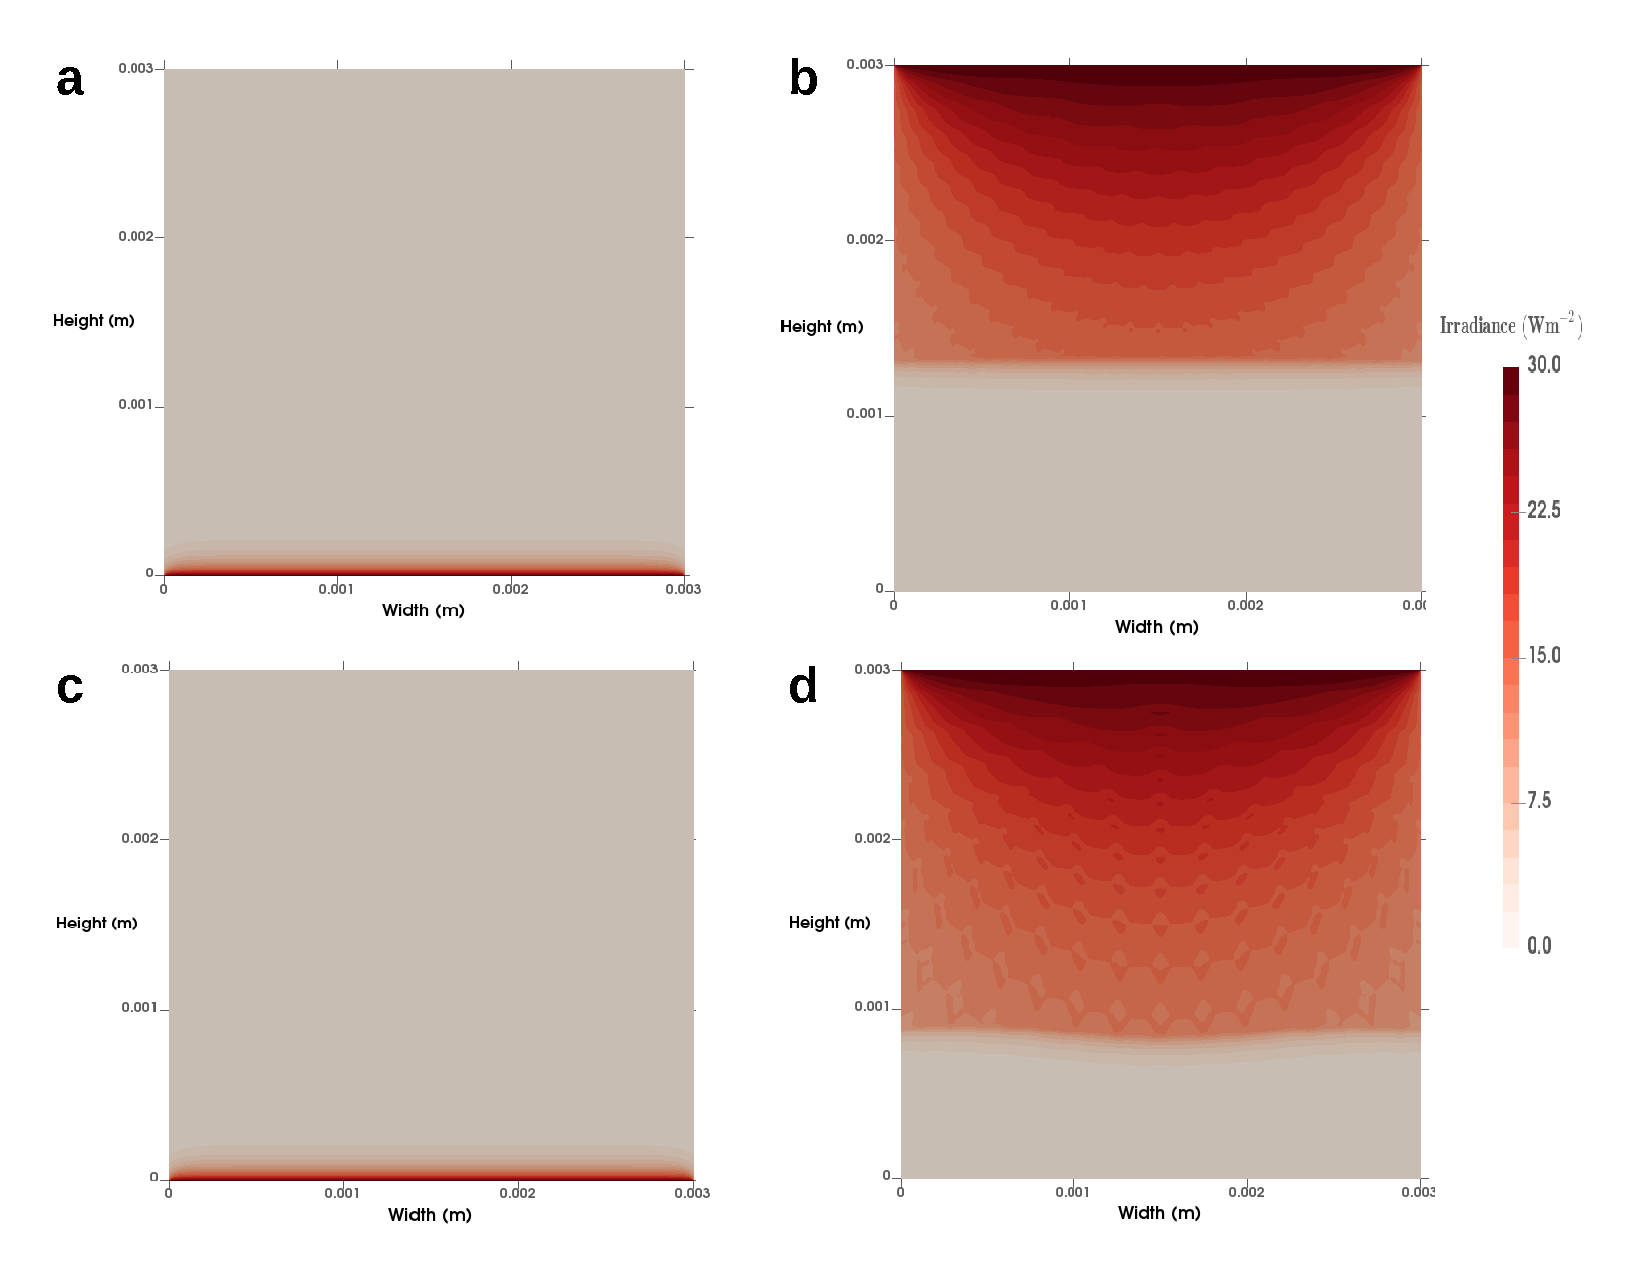
\includegraphics[width=\textwidth]{Chap4/results/biofilm_process.pdf}
    \caption{Graphical presentation of the lifecycle of a biofilm.} 
    \label{fig:biofilm_processes}
\end{figure}


\subsubsection{Examples of beneficial and harmful biofilms}
It is important to understand the mechanisms of biofilm formation, whether the biofilm be beneficial or harmful. Examples of beneficial biofilms in process engineering applications include for the bioremediation of contaminated soils \cite{singh2006} and wastewater treatment applications where nutrients and impurities are removed from water streams through trickling filters or other engineered designs. Another application of interest in biotechnology is where biofilms aid in the harvesting of protein-rich bacteria, effectively short-cutting the need for expensive separation equipment associated with biomass thickening and dewatering \cite{hulsen2016a}.
\skippingparagraph
On the other hand, bad biofilms can also have such effects as reducing process equipment efficiency, being dangerous, harmful, or completely pernicious \cite{donlan2002}. Examples include the fouling on heat transfer and membrane equipment leading to a reduction in process performance \cite{mcdonogh1994}, the formation of biofilms in food cultivation and preparation areas \cite{wirtanen2003}. The control of biofilms is vitally important in the health industry, as they present themselves as sources for inflammation, impaired healing, antimicrobial resistance, and patient death \cite{bryers2008}. As biofilm formation and growth can have significant positive or negative effects on society, the modelling of these systems is important in order to understand the details of the governing processes, therefore prevail in controlling such formation in practical applications. 


\subsubsection{Modelling of biofilms}
The current state of progress in biofilm modelling is where heterogeneity and spatio-temporal variations are described within the model. The complex nature of biofilms, and the ever increasing access to significant computational power means that it is logistically becoming easier to implement these complex models. They are known as third generation models according to the IWA's task group on biofilm modelling. They build on the previous classes of biofilm modelling where steady-state, homogeneous biofilms were defined in order to describe mass transport between biofilm and bulk flow (first generation) \cite{wanner2006}. Second generation models included updates to account for non-uniformities in the biofilm by describing microbial interactions. Third generation models can be described as either based on discrete agents, or as continuum models \cite{dacunto2017}. Each approach has its own benefits and drawbacks.\\

\textbf{Discrete agent biofilm models}\\
There are two major discrete modelling approaches for biofilm formation: cellular automaton and agent based models. Cellular automaton models consist of discretising the spatial domain into discrete squares or cuboids for 2D or 3D models respectively. Each discrete element can be either occupied by a microbial cell, or a substance of interest, or can be empty. The cells are subjected to simple, discrete biological or physical operations \cite{dacunto2017}. The operations, or rules, can include substrate diffusion, biokinetics expressions such as growth and decay, and attachment and detachment processes \cite{skoneczny2015}. Broadly accepted advantages of cellular automaton (CA) approaches are that the model setup oftentimes offers a simpler  development cycle as it is based on a series of discrete steps. In addition, the implementation of irregular boundary conditions is easier with this method \cite{pizzaro2001}, and the approach is known to be relatively simple to implement across multiple computing processors when compared to differential descriptions of states \cite{toffoli1987} . There are several disadvantages to the CA method, including the fact that conservation is not maintained under substrate uptake and growth processes, and the biofilm advances based on the availability of unoccupied cells. This means that dynamic growth and transformation processes closer to the substratum are often ignored \cite{dacunto2017}. Additionally, as cells are effectively placeholders for physical information, the mesh cells are often of uniform physical state. The accuracy is therefore dependent on the resolution of the meshed domain \cite{dacunto2017}.
\skippingparagraph
The other main method of discrete biofilm modelling is the agent based modelling (ABM) approach. This technique is similar to the CA approach insofar as it incorporates a set of rules that biomass follows. However, it differs in that the representation of biofilm species is as particulate matter, which can occupy any point in continuous spaces. Constraints due to the discretised CA lattice do not apply. Agent based models have been used to describe the interactions between multispecies particulates, including EPS formation and its effects on the the biofilm structure \cite{xavier2005a}. As the physical complexity of the modelled biofilm system increases, brute-force ABM simulations of complex systems often encounter computational limitations, limiting the spatial scale of ABMs. To overcome this limitation larger particles representing fractions of inert and active biomass has been presented. This type of model still follows ABM methods, with free-flowing particles, but the particles act as aggregate placeholders for physical information, similar to the CA methods \cite{picioreanu2004}.
\skippingparagraph
Discrete approaches allow for the construction of complex models by building series of simple constraining rules. Model results often lead to a general idea of how the biofilm structure is formed, however agreement with experimental data is frequently case-specific \cite{dacunto2017}. This is due to the description of the physical phenomena being based on a set of simple instructions with aspects of stochasticity. The order in which these instructions are executed can influence the results of the model, as well as the random nature of the discrete operations mean that results from identical initial conditions can differ significantly. Consequently, rigorous statistical analysis must be conducted in order to confirm the results from discrete models \cite{alpkvist2006}.\\

\textbf{Continuum-based biofilm models}\\
Continuum-based biofilm models can be classed into two main categories; one dimensional models (1D) and multidimensional models (2D for domains in $\mathbb{R}^2$-space and 3D for domains in $\mathbb{R}^3$-space respectively). Perhaps the most widely used 1D biofilm model is the AQUASIM implementation \cite{reichert1994} which builds upon the groundwork of \cite{wanner1986} \cite{wanner1986}. This model considers a multispecies competition and distribution within a biofilm. Included in the model are attachment and detachment processes, as well as considerations of mass transfer of soluble substrates within the porous structures. 1D biofilm model best lend themselves to particular cases: \textit{i)} in educational or demonstration settings, \textit{ii)} as part of broader or plant-wide models where mass exchange between biofilms and soluble substrates is to be quantified, but where computational requirements are to be used sparingly \cite{dacunto2017}.
\skippingparagraph
Multidimensional biofilm models are able to capture non-uniformities in the plan parallel to the surface substratum. Through this approach, one can explore the interactions between several species within a biofilm. Also, 2D and 3D approaches allow for analysis of time and space-dependent physical parameters and variables such as species and other particulate distribution, pressure gradients, and the interactions between soluble species and the porosity of the biofilm structure \cite{eberl2001}. Demonstrations in 1D and 3D test cases with varying symmetric and asymmetric boundary conditions were run, and the assessment of biofilm growth was found to agree well with experimental results. \cite{alpkvist2007}, (\cite{alpkvist2007}) also recognised the limitations associated with discrete models or 1D continuum models and thus proposed an extension to the Wanner-Gujer model as implemented in AQUASIM \cite{wanner1986}. The model linked a biomass volume fraction to Monod growth kinetics. The changes in volume fraction described changes in pressure which was the driver of biomass spreading. As the biofilm front represented a boundary and was dynamic, interface capturing was achieve with the level-set method, which allows for the reconstruction of the biomass front from a differential distance function. 2D and 3D simulations were carried out, and the results showed the formation of microbial niches due to substrate gradients. This model represents one of the first examples of a mathematically rigorous approach being taken to biofilm modelling.
\skippingparagraph

\textbf{Photobiofilm models}\\
As the field of study of photobioreactors is in its infancy, the benefits of photobiofilm reactors have seldom been discussed. It has been identified that the harvesting, thickening and dewatering costs associated with phototrophic processes could be reduced if growth by attachment was the dominant growth mode in photobioreactors  \cite{hulsen2016a}. Purple phototrophic bacteria (PPB) are known to form heterogeneous, somewhat stratified biofilm structures in benthic zones of aquatic environments \cite{overmann2013}, however algal biomass has proven more difficult to engineer into biofilm formations. A recent attempt to foster a mycoalgal biofilm proved to be more effective than in the axenic cultures \cite{rajendran2016}, but for applications such as waste treatment, one doesn't have the privilege of being able to select specific co-cultures. That said, whatever the application of photobiofilm systems, that elucidation of the process kinetics coupled with biofilm development is required for a deeper understanding, especially with respect the coupling with the radiative field.
\skippingparagraph
With regards to phototrophic biofilm modelling, only two examples exist prior to this work. The first phototrophic biofilm (PBF) model was proposed as a two dimensional application to a porous susbstrate photobioreactor (PSBR) \cite{murphy2014}. The model looked at the productivity of \textit{Anabaena variabilis}, a cyanobacterium, through substrate transport, photon delivery, and growth processes. There was good agreement between numerical simulations and experimental results with respect to biomass productivity over a range of thicknesses between 35 \SI{}{\micro\metre} and 46 \SI{}{\micro\metre}. This model focused on a pure culture of cyanobacteria, and the evolution of biofilm structure was not explored in this scope. Additionally, variations in soluble substrate concentrations into the biofilm towards the surface substratum were not presented. 
\skippingparagraph
The second study focused on a 1D application of a PBSR \cite{li2016}. This model extended the previously mentioned study with respect to the substrate gradients perpendicular to the biofilm surface substratum. The radiative transfer equation was used to simulate the light delivery to the biofilm concluded that phase in-scattering and pigment adaptation were important considerations. The advection of the biofilm front was by treating the biomass length as a discrete quantity, either consuming or releasing discrete elements at each simulated time step. \skippingparagraph


%------------------------------------------------------------------------------%
%------------------------------------------------------------------------------%
\section{Research objectives and approach}
\label{Intro:Objectives}
Several research gaps have been determined in response to the suite of literature available since the beginning of this thesis. Photosynthesis process modelling techniques are generally well understood, especially when developed and validated against artificially irradiated photobioreactors. Biological process models fall into three main categories, labelled type I, II, and III \cite{bechet2013}. These categories relate to their degree of complexity, especially when growth expressions are coupled to the radiative field. Type I models assume that all photosynthetic organisms are irradiated uniformly with an irradiance equal to that of the irradiated surface of a photobioreactor or the averaged irradiance within a solution domain. Type II models aim to decompose a solution domain into several subdomains of uniform irradiance. This means that the growth and productivity of a photosynthetic system can be described in terms of a light gradient. Type III models assess the light history of a photosynthetic particle, and describe the growth behaviour as the particles flow in and out of irradiated areas within a photobioreactor. This third type of model requires a description of the flow field as well as a light gradient to accurately determine biomass growth. Biological growth terms can consider either the photosynthetic microorganisms as a bulk single state, or as three different states depending on the perceived irradiance of the particles \cite{eilers1988}. The latter biological model is the most widely used within process models for photosynthetic productivity. Despite the rich suite of process modelling and computational fluid dynamics approaches for algal biomass, there is no equivalent for purple phototrophic bacteria. With different metabolisms to those of algae, it is not sufficient to base PPB models off algal models. However, these can serve as inspiration when developing spatiotemporal models.

\subsection{Research objective 1: A description of the process biokinetics of phototrophic systems}
The growth of PPB in a nutrient rich environment has not been described at the process level. With limitations such as non-trivial requirements for light energy, mixing energy, and harvesting challenges, a model with a higher level of abstraction than a metabolic pathway description is required.

A photo-anaerobic model (PAnM) was developed to address these concerns. The model was based on the IWA semi-mechanistic family of models and used Monod expressions for nutrient and light limitations. The model was designed such that extension to three spatial dimensions was possible. 

\subsection{Research objective 2: Computational fluid dynamics analysis of single and two-phase photobioreactors}
Based on the literature review, photosynthetic and phototrophic systems vary in space as well as time, due to irradiation and fluid flows. While algal CFD models have already been applied, few considered a coupled multiphysics solution, and the solution work flow of coupled solution procedures has been disjointed, with multiple simulation environments being used for models. 

A modelling framework was therefore developed in OpenFOAM which included the coupling between single or multiphase flows, radiative transfer, and biokinetic behaviour of the phototrophic biomass.

\subsection{Research objective 3: A multidimensional, phototrophic, continuum biofilm model}
The harvesting of phototrophic biomass presents challenges as separation processes and technologies such as membrane bioreactors can be expensive both in terms of operational and capital expenditure. A potential method to remove biomass from a multiphase system is to grow it attached on surfaces, and mechanically scrape the bacterial community from those surfaces as single solid biomass. Research objectives 1 and 2 which look at the definition of the photo-biological reactions and the corresponding lumped parameter system respectively form a basis for exploring biofilm growth. 

A phototrophic biofilm model was developed which looked at the growth of mixed phototrophic biomass as it grows from an irradiated substratum. 





